\chapter{Gerarchia delle classi}

\section{MainActivity}
\begin{figure}[ph]
	\centering
	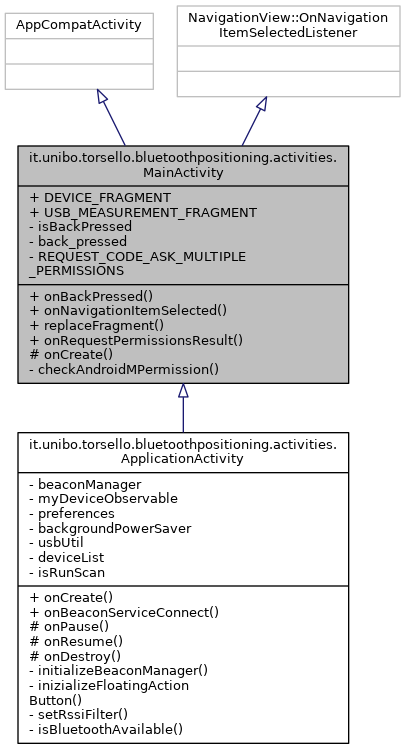
\includegraphics[width=0.40\linewidth]{img/uml/class/classit_1_1unibo_1_1torsello_1_1bluetoothpositioning_1_1activities_1_1MainActivity__inherit__graph.png}
	\caption{Classe - MainActivity}
\end{figure}
La classe \texttt{Main} viene istanziata per prima all'avvio dell'app. Serve ad inizializzare gli oggetti grafici, controllare la compatibilità con Android 5.0+ e rimpiazzare i fragment da visualizzare selezionati dal menu a sinistra.

\begin{figure}[ph]
	\centering
	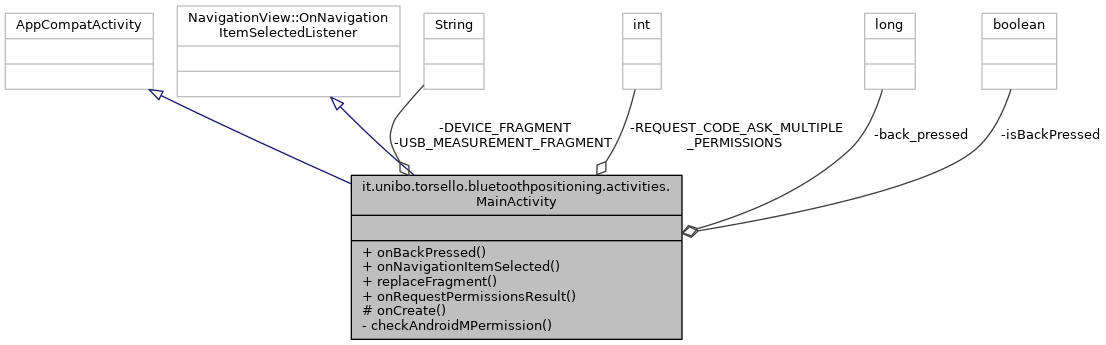
\includegraphics[width=1.8\linewidth,angle=90]{img/uml/class/classit_1_1unibo_1_1torsello_1_1bluetoothpositioning_1_1activities_1_1MainActivity__coll__graph.png}
	\caption{Collaborazione - MainActivity}
\end{figure}

\newpage
\section{ApplicationActivity}
\begin{figure}[ph]
	\centering
	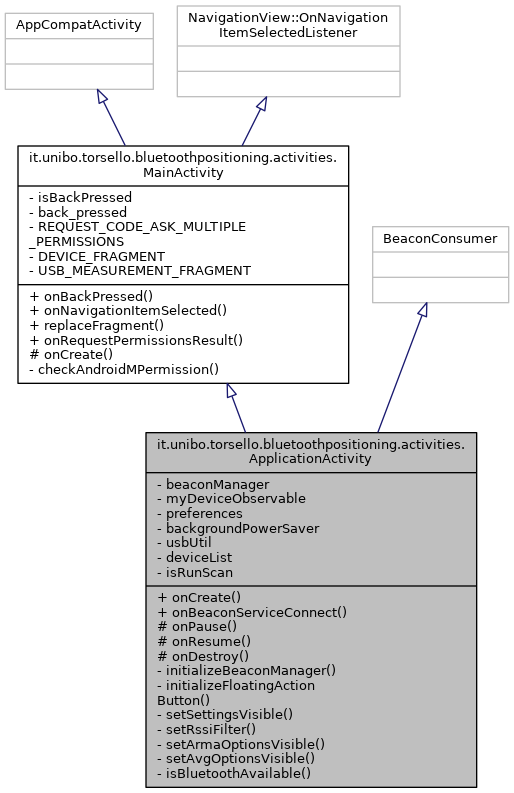
\includegraphics[width=0.7\linewidth]{img/uml/class/classit_1_1unibo_1_1torsello_1_1bluetoothpositioning_1_1activities_1_1ApplicationActivity__inherit__graph.png}
	\caption{Classe - ApplicationActivity}
\end{figure}

Questa classe è una parte fondamentale del progetto. Qui si istanzia e controlla l'oggetto \texttt{BeaconManager} responsabile dello scanning su BT e quindi si ricevono le informazioni dei dispositivi vicini.

Alla ricezione dei dati, questi vengono spediti al \texttt{DeviceObservable} a cui tutti gli Observer interessati si registreranno in modo da ottenere tutti lo stesso valore aggiornato.

\begin{figure}[ph]
	\centering
	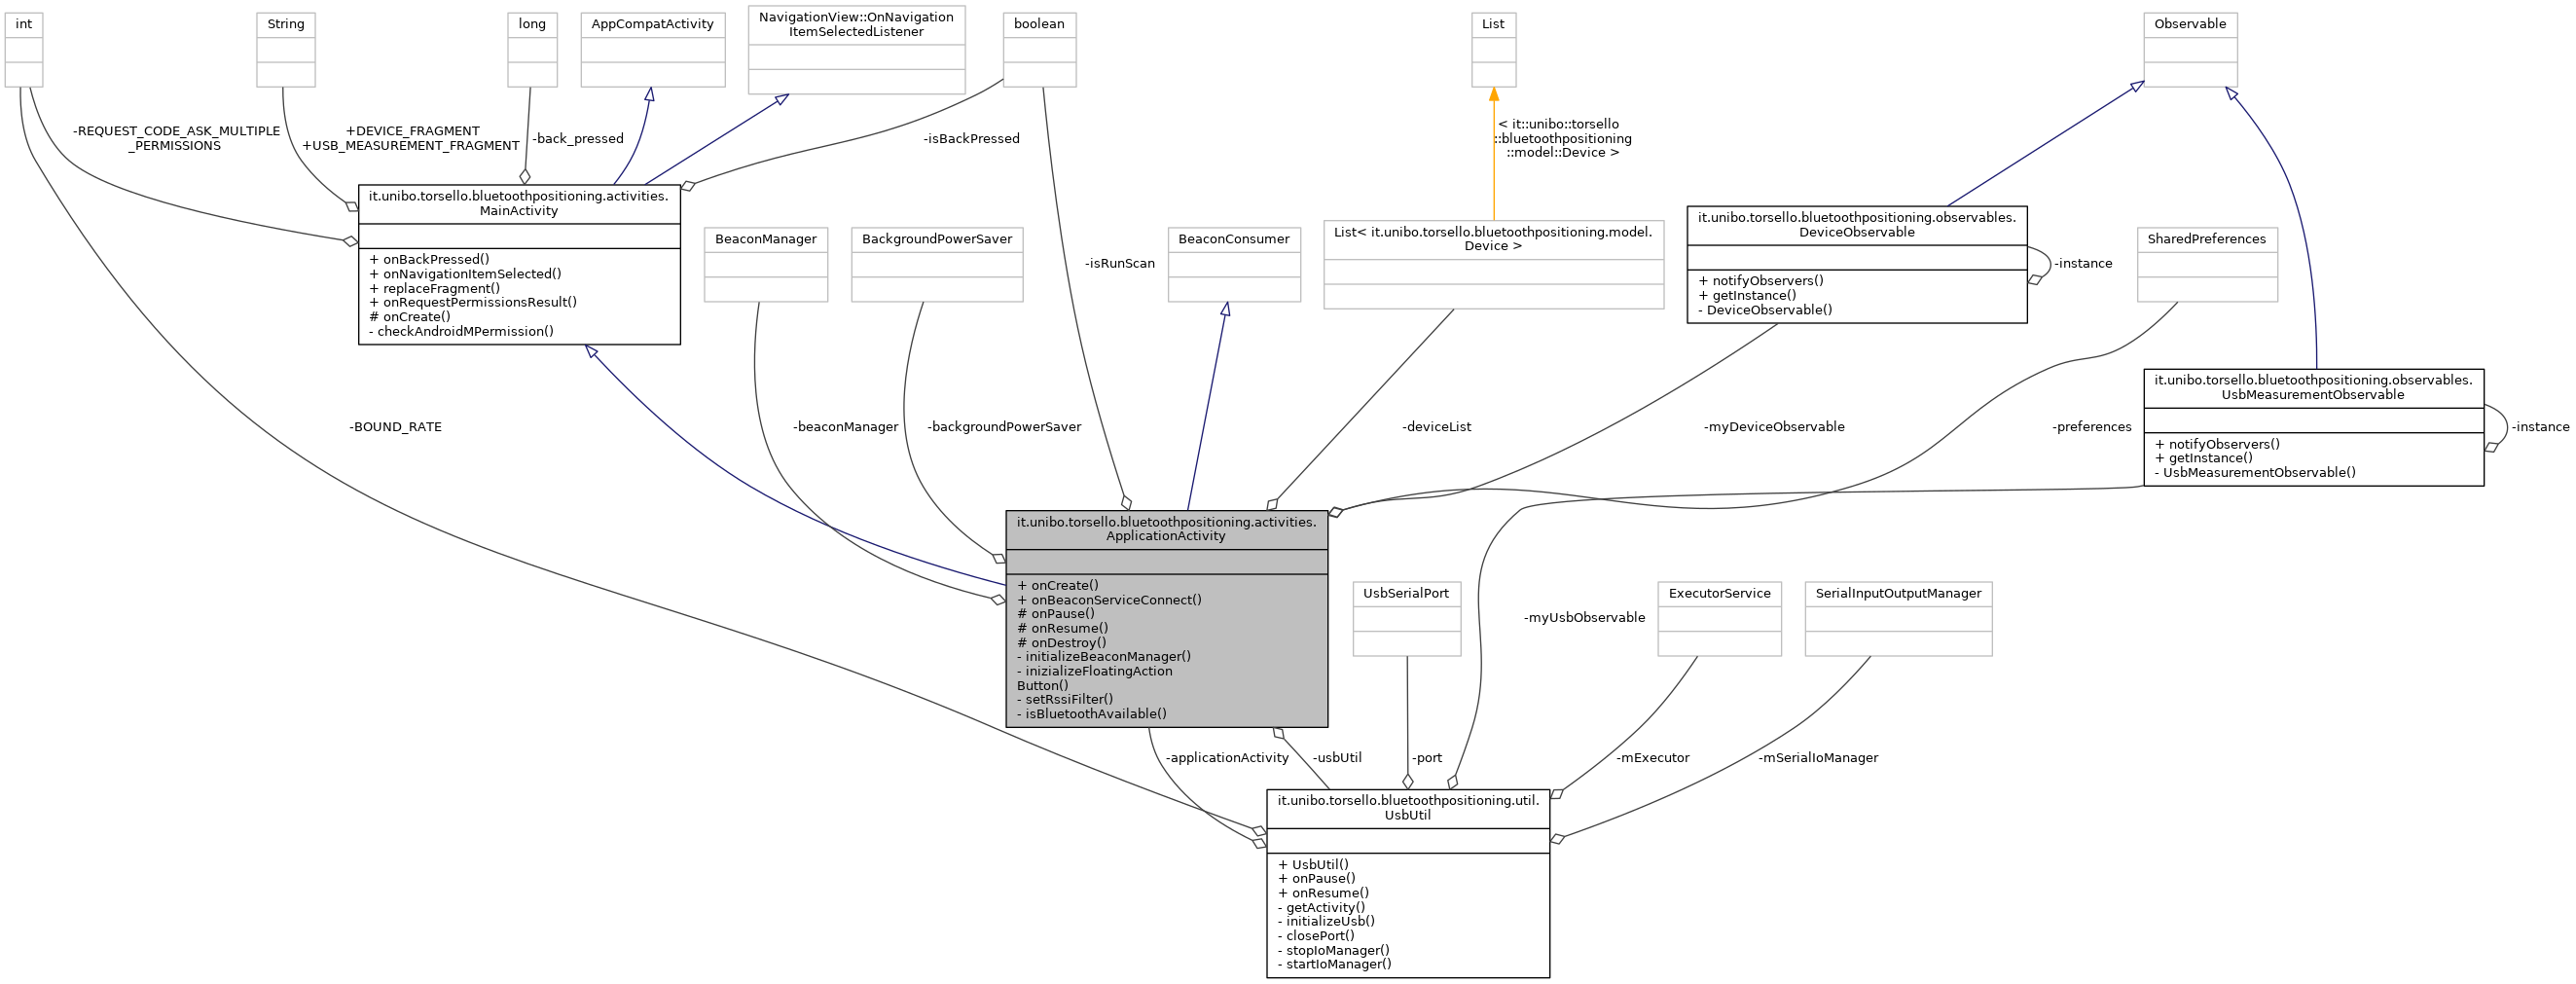
\includegraphics[width=1.9\linewidth, angle=90]{img/uml/class/classit_1_1unibo_1_1torsello_1_1bluetoothpositioning_1_1activities_1_1ApplicationActivity__coll__graph.png}
	\caption{Collaborazione - ApplicationActivity}
\end{figure}

\newpage
\section{Device}
\begin{figure}[ph]
	\centering
	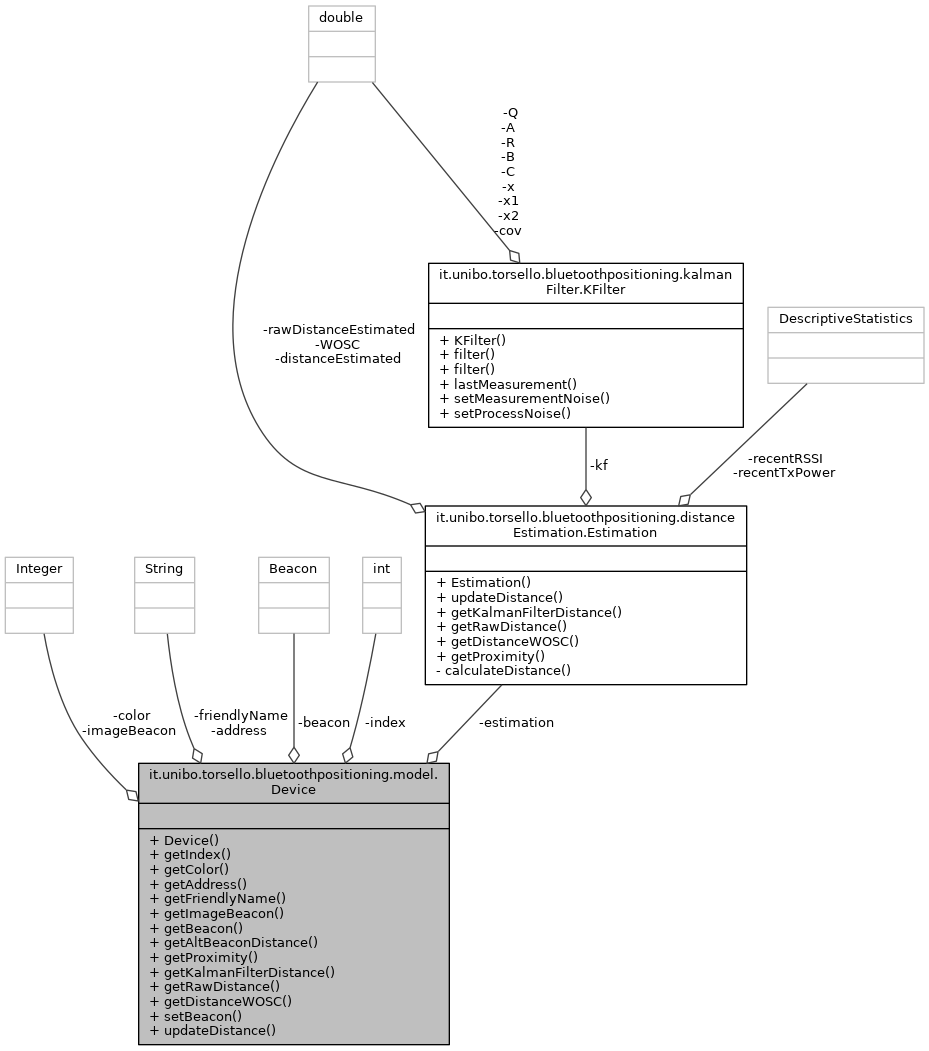
\includegraphics[width=0.9\linewidth]{img/uml/class/classit_1_1unibo_1_1torsello_1_1bluetoothpositioning_1_1model_1_1Device__coll__graph.png}
	\caption{Collaborazione - Device}
\end{figure}

Classe che modella la definizione di dispositivo Bluetooth BLE nel sistema. Alcuni dei dati presenti nella classe sono inizializzati alla creazione che avviene nella classe \texttt{DeviceConstants}, altri sono invece calcolati durante l'esecuzione, come la stima della distanza da parte dei vari filtri.

\newpage
\section{DeviceConstants}
\begin{figure}[ph]
	\centering
	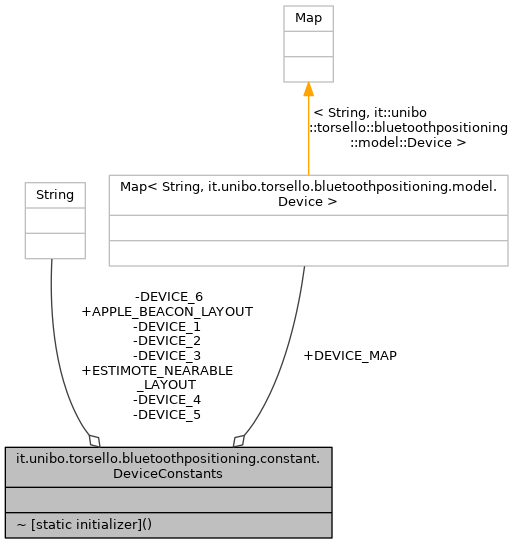
\includegraphics[width=0.7\linewidth]{img/uml/class/classit_1_1unibo_1_1torsello_1_1bluetoothpositioning_1_1constant_1_1DeviceConstants__coll__graph.png}
	\caption{Collaborazione - DeviceConstants}
\end{figure}

Classe che modella ed inizializza i dispositivi sotto forma di oggetto \texttt{Device}. Al suo interno è presente una \texttt{Map} in cui sono indicati i soli ed unici dispositivi che saranno riconosciuti dal sistema.

\newpage
\section{DeviceObservable}
\begin{figure}[ph]
	\centering
	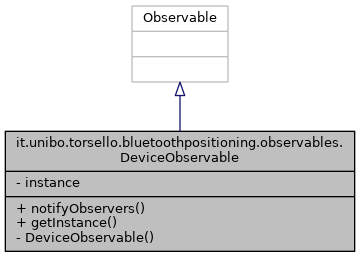
\includegraphics[width=0.7\linewidth]{img/uml/class/classit_1_1unibo_1_1torsello_1_1bluetoothpositioning_1_1observables_1_1DeviceObservable__inherit__graph.png}
	\caption{Classe - DeviceObservable}
\end{figure}

Lo scopo di questa classe è creare un Observable che notifichi a tutti gli Observer registrati l'oggetto list con tutti gli update dei dispositivi scansionati. Questa lista viene aggiornata nella classe \texttt{ApplicationActivity} nel metodo \texttt{onBeaconServiceConnect}

\newpage
\section{Estimation}
\begin{figure}[ph]
	\centering
	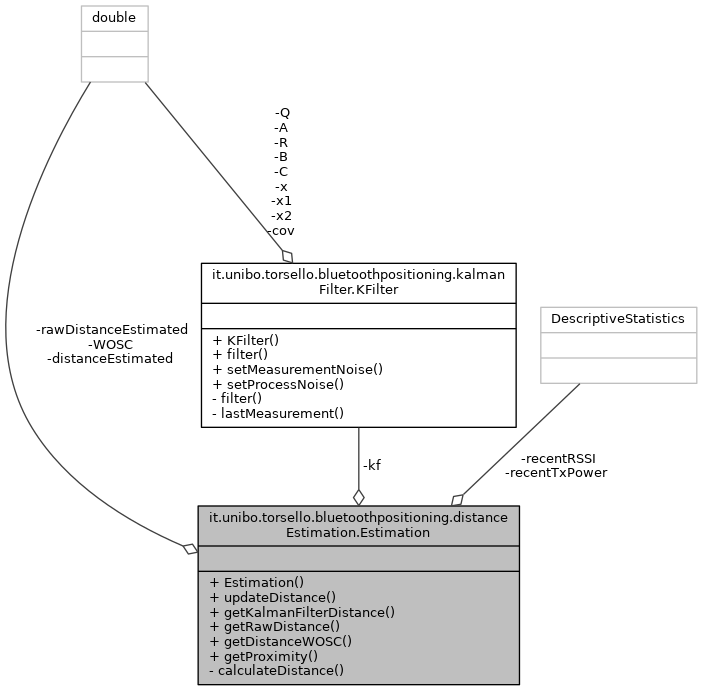
\includegraphics[width=1.2\linewidth]{img/uml/class/classit_1_1unibo_1_1torsello_1_1bluetoothpositioning_1_1distanceEstimation_1_1Estimation__coll__graph.png}
	\caption{Collaborazione - Estimation}
\end{figure}

\newpage
\section{SettingsFragment}
\begin{figure}[ph]
	\centering
	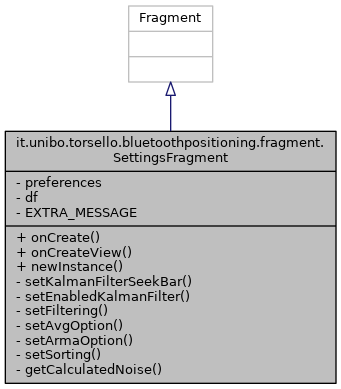
\includegraphics[width=0.5\linewidth]{img/uml/class/classit_1_1unibo_1_1torsello_1_1bluetoothpositioning_1_1fragment_1_1SettingsFragment__inherit__graph.png}
	\caption{Classe - SettingsFragment}
\end{figure}

Classe che implementa Fragment per creare una vista disposta in un menu a destra. Il suo scopo è permettere all'utente di interagire con l'app e con il sistema fisico in cui ci si esegue la stima modificando dei semplici parametri.

\newpage
Nel particolare si usa l'oggetto \texttt{SharedPreferences} per salvare le impostazioni utilizzate. Nel caso in cui l'app fosse chiusa, le impostazioni salvate precedentemente vengono reimpostate come se l'app non fosse mai stata terminata.

\begin{figure}[ph]
	\centering
	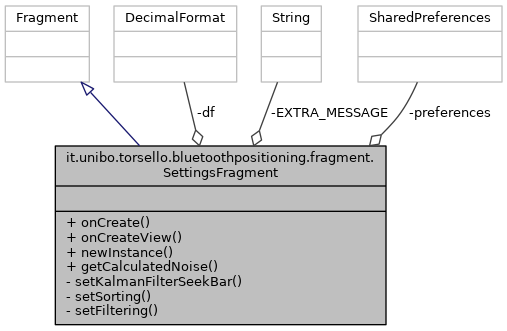
\includegraphics[width=0.8\linewidth]{img/uml/class/classit_1_1unibo_1_1torsello_1_1bluetoothpositioning_1_1fragment_1_1SettingsFragment__coll__graph.png}
	\caption{Collaborazione - SettingsFragment}
\end{figure}

\newpage
\section{SettingConstants}

Classe in cui si settano le costanti relative ai settaggi. Tali costanti sono intese come chiavi per risalire alle impostazioni scelte dall'utente, come ad esempio il filtro o l'ordinamento dei dispositivi trovati.
\begin{figure}[ph]
	\centering
	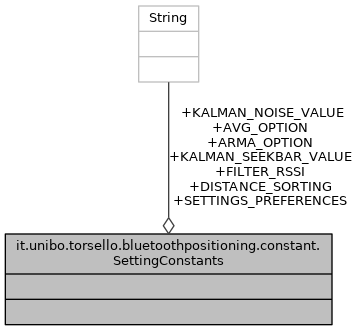
\includegraphics[width=0.5\linewidth]{img/uml/class/classit_1_1unibo_1_1torsello_1_1bluetoothpositioning_1_1constant_1_1SettingConstants__coll__graph.png}
	\caption{Collaborazione - SettingConstants}
\end{figure}

\newpage
\section{DeviceListFragment}\label{ch:device_list}
\begin{figure}[ph]
	\centering
	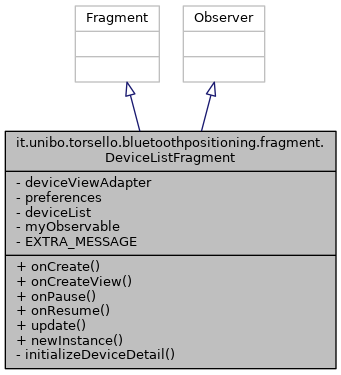
\includegraphics[width=0.5\linewidth]{img/uml/class/classit_1_1unibo_1_1torsello_1_1bluetoothpositioning_1_1fragment_1_1DeviceListFragment__inherit__graph.png}
	\caption{Classe - DeviceListFragment}
\end{figure}

Classe che aggiorna la lista dei dispositivi con le nuove informazioni ricevute dal metodo \texttt{update(...)}, \textit{override} della classe Observer.
\begin{lstlisting}[language=Java]
@Override
publilc void update(Observable o, Object arg) {
	
	if (arg instanceof List) {
		
		if (!deviceList.isEmpty()) {
			deviceList.clear();
		}
		
		List<Device> devices = (List<Device>) arg;
		
		// optional sorting
		Collections.sort(devices, new Comparator<Device>() {
			public int compare(Device b1, Device b2) {
				int sorting = preferences
					.getInt(SettingConstants.DISTANCE_SORTING, 0);
				switch (sorting) {
					case 0:
					case R.id.radioButton_default_sorting:
					return Double.compare(b1.getIndex(), b2.getIndex());
					case R.id.radioButton_color_sorting:
					return Double.compare(b1.getColor(), b2.getColor());
					case R.id.radioButton_distance_sorting:
					return Double.compare(b1.getKalmanFilterDistance(), b2.getKalmanFilterDistance());
				} // default sorting (a good basic ordering for the other options)
				return Double.compare(b1.getIndex(), 
						b2.getIndex());
			}
		});
		
		deviceList.addAll(devices);
		deviceViewAdapter.notifyDataSetChanged();
	}
}
\end{lstlisting}

Nel dettaglio si aggiorna la lista in base alle preferenze impostate in \texttt{Settings}.

\begin{figure}[ph]
	\centering
	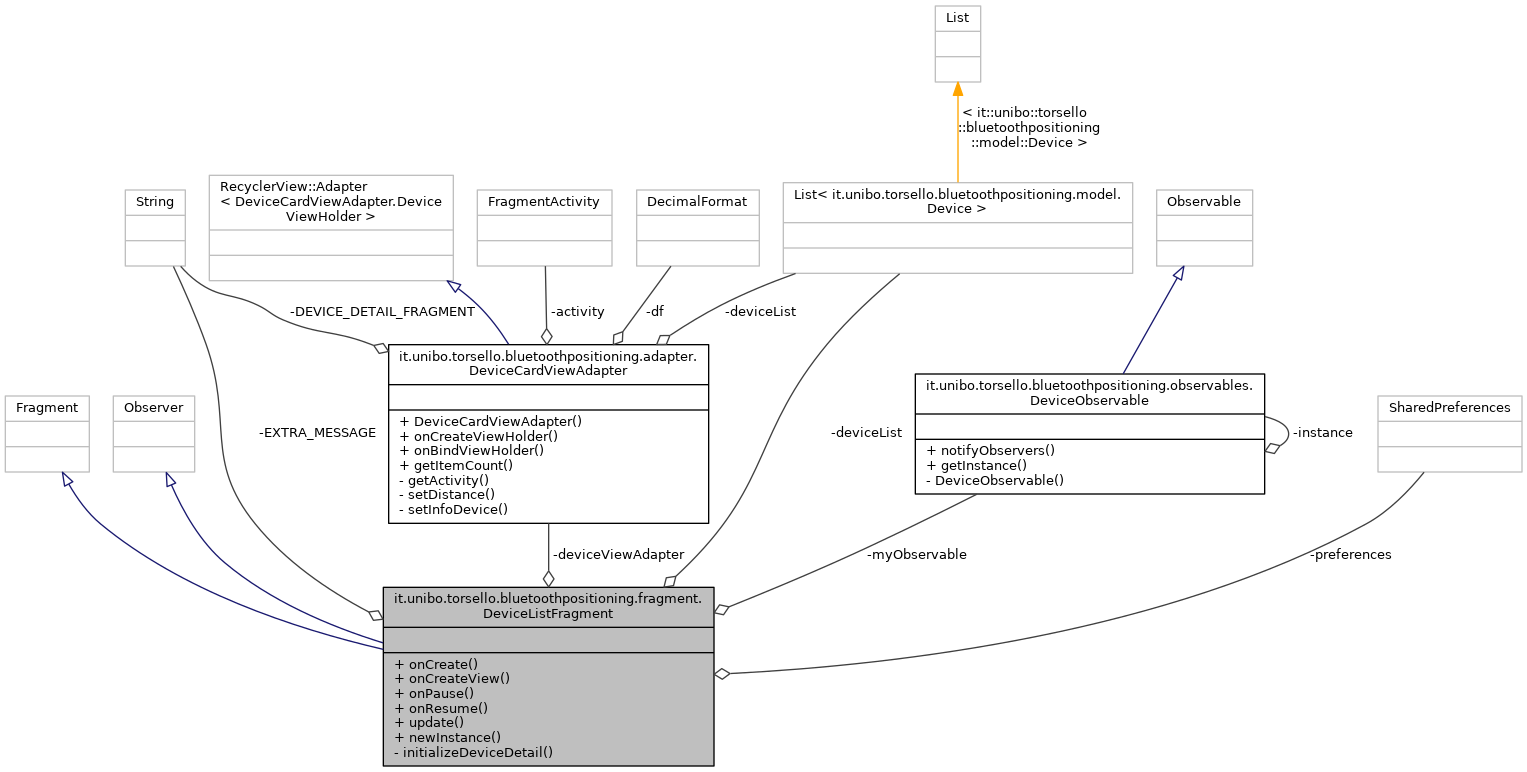
\includegraphics[width=1.6\linewidth,angle=90]{img/uml/class/classit_1_1unibo_1_1torsello_1_1bluetoothpositioning_1_1fragment_1_1DeviceListFragment__coll__graph.png}
	\caption{Collaborazione - DeviceListFragment}
\end{figure}

\newpage
\section{DeviceCardViewAdapter}
\begin{figure}[ph]
	\centering
	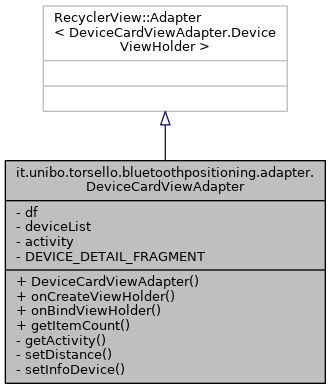
\includegraphics[width=0.5\linewidth]{img/uml/class/classit_1_1unibo_1_1torsello_1_1bluetoothpositioning_1_1adapter_1_1DeviceCardViewAdapter__inherit__graph.png}
	\caption{Classe - DeviceCardViewAdapter}
\end{figure}

Classe responsabile della visualizzazione delle nuove informazioni a schermo. Qui si gestiscono gli elementi grafici da fare vedere o nascondere (valori testuali o immagini) nella RecyclerView.

Viene utilizzata nella schermata principale e nel fragment dei dettagli.

\begin{figure}[ph]
	\centering
	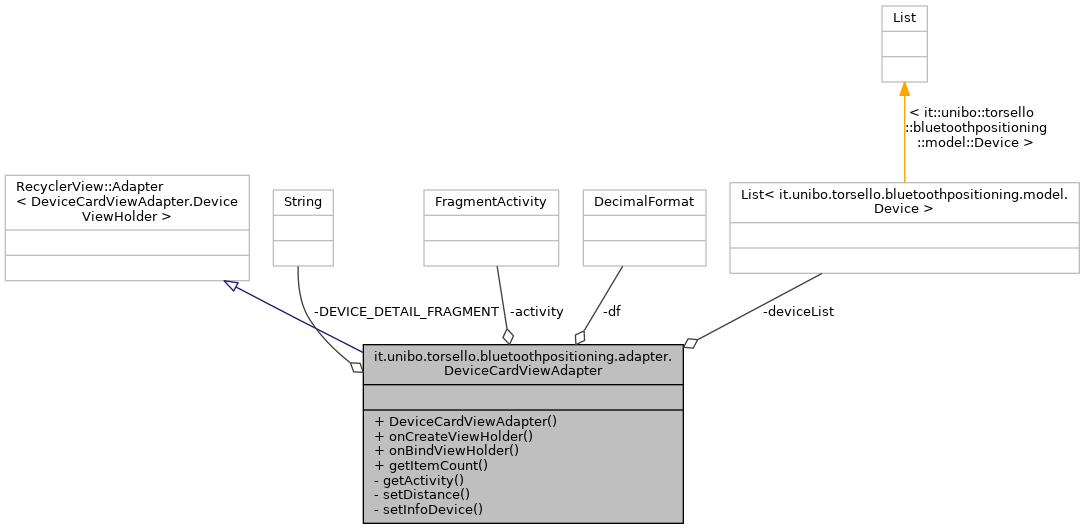
\includegraphics[width=1.5\linewidth,angle=90]{img/uml/class/classit_1_1unibo_1_1torsello_1_1bluetoothpositioning_1_1adapter_1_1DeviceCardViewAdapter__coll__graph.png}
	\caption{Collaborazione - DeviceCardViewAdapter}
\end{figure}

\newpage
\section{DeviceViewHolder}
\begin{figure}[ph]
	\centering
	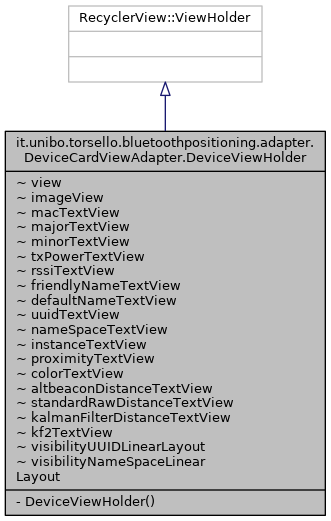
\includegraphics[width=0.5\linewidth]{img/uml/class/classit_1_1unibo_1_1torsello_1_1bluetoothpositioning_1_1adapter_1_1DeviceCardViewAdapter_1_1DeviceViewHolder__inherit__graph.png}
	\caption{Classe - DeviceViewHolder}
\end{figure}

Classe che serve ad inizializzare i vari oggetti grafici da visualizzare nel RecyclerView, risparmiando memoria.

\begin{figure}[ph]
	\centering
	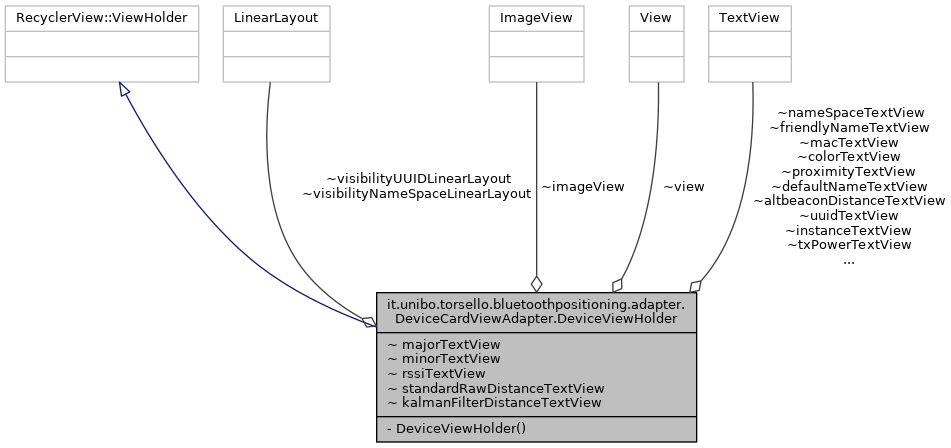
\includegraphics[width=1.5\linewidth,angle=90]{img/uml/class/classit_1_1unibo_1_1torsello_1_1bluetoothpositioning_1_1adapter_1_1DeviceCardViewAdapter_1_1DeviceViewHolder__coll__graph.png}
	\caption{Collaborazione - DeviceViewHolder}
\end{figure}

\newpage
\section{MyArmaRssiFilter}
\begin{figure}[ph]
	\centering
	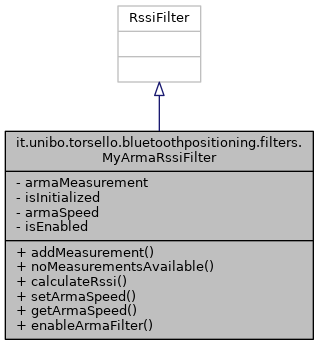
\includegraphics[width=0.5\linewidth]{img/uml/class/classit_1_1unibo_1_1torsello_1_1bluetoothpositioning_1_1filters_1_1MyArmaRssiFilter__inherit__graph.png}
	\caption{Classe - MyArmaRssiFilter}
\end{figure}

Classe in cui si esegue il filtraggio ARMA spiegato in \ref{ch:filtro_arma}.

\begin{figure}[ph]
	\centering
	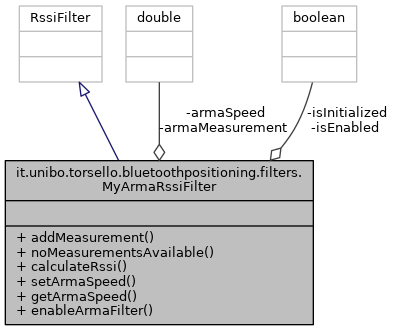
\includegraphics[width=0.65\linewidth]{img/uml/class/classit_1_1unibo_1_1torsello_1_1bluetoothpositioning_1_1filters_1_1MyArmaRssiFilter__coll__graph.png}
	\caption{Collaborazione - MyArmaRssiFilter}
\end{figure}

\newpage
\section{KFilterBuildertFragment}
Classe di supporto per la creazione di un \texttt{KFilter}. Il suo scopo è inizializzare tale oggetto con dei parametri passati al costruttore.
\begin{figure}[ph]
	\centering
	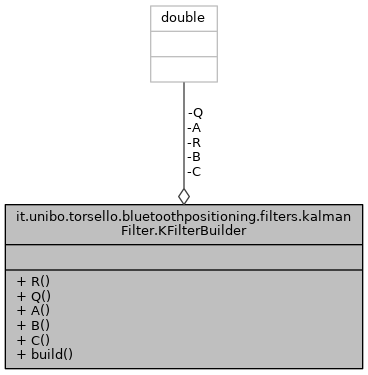
\includegraphics[width=0.6\linewidth]{img/uml/class/classit_1_1unibo_1_1torsello_1_1bluetoothpositioning_1_1filters_1_1kalmanFilter_1_1KFilterBuilder__coll__graph.png}
	\caption{Collaborazione - KFilterBuildertFragment}
\end{figure}

\newpage
\section{KFilter}

Classe per l'implementazione del filtro di Kalman. Il suo funzionamento viene spiegato in \ref{ch:kfilter}.

\begin{figure}[ph]
	\centering
	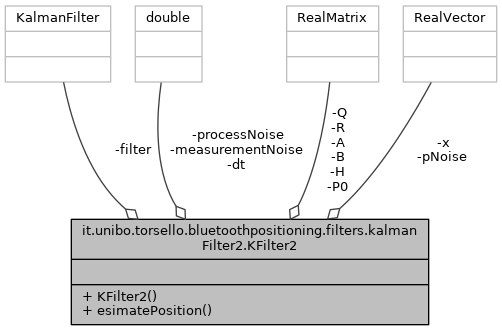
\includegraphics[width=0.8\linewidth]{img/uml/class/classit_1_1unibo_1_1torsello_1_1bluetoothpositioning_1_1filters_1_1kalmanFilter2_1_1KFilter2__coll__graph.png}
	\caption{Collaborazione - KFilter}
\end{figure}

\newpage
\section{KFilterConstants}
\begin{figure}[ph]
	\centering
	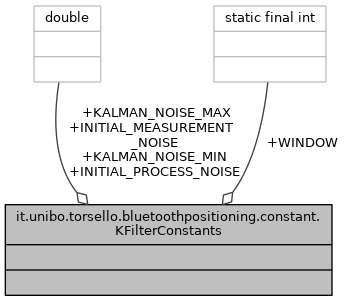
\includegraphics[width=0.6\linewidth]{img/uml/class/classit_1_1unibo_1_1torsello_1_1bluetoothpositioning_1_1constant_1_1KFilterConstants__coll__graph.png}
	\caption{Collaborazione - KFilterConstants}
\end{figure}

\newpage
\section{StatePagerAdapter}
\begin{figure}[ph]
	\centering
	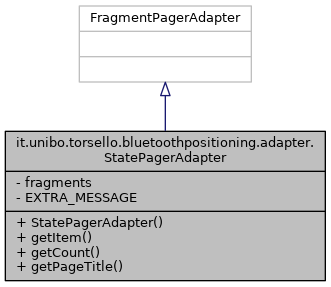
\includegraphics[width=0.5\linewidth]{img/uml/class/classit_1_1unibo_1_1torsello_1_1bluetoothpositioning_1_1adapter_1_1StatePagerAdapter__inherit__graph.png}
	\caption{Classe - StatePagerAdapter}
\end{figure}

Questa classe estende FragmentPagerAdapter per creare un ambiente in cui aggiungere i fragment dei dettagli riguardanti i beacon.

\begin{figure}[ph]
	\centering
	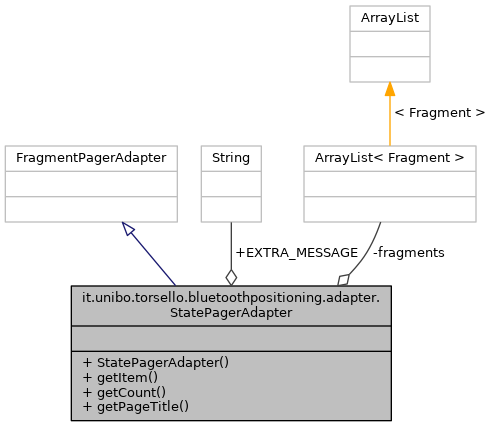
\includegraphics[width=0.75\linewidth]{img/uml/class/classit_1_1unibo_1_1torsello_1_1bluetoothpositioning_1_1adapter_1_1StatePagerAdapter__coll__graph.png}
	\caption{Collaborazione - StatePagerAdapter}
\end{figure}

\newpage
\section{DeviceDetailFragment}
\begin{figure}[ph]
	\centering
	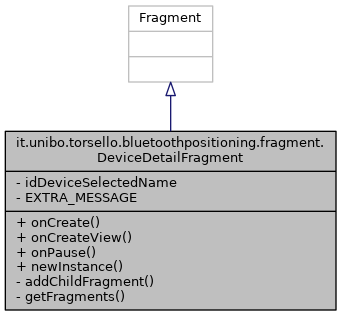
\includegraphics[width=0.5\linewidth]{img/uml/class/classit_1_1unibo_1_1torsello_1_1bluetoothpositioning_1_1fragment_1_1DeviceDetailFragment__inherit__graph.png}
	\caption{Classe - DeviceDetailFragment}
\end{figure}

Classe che istanzia \texttt{StatePagerAdapter} per aggiunge i fragment dei dettagli.

\begin{figure}[ph]
	\centering
	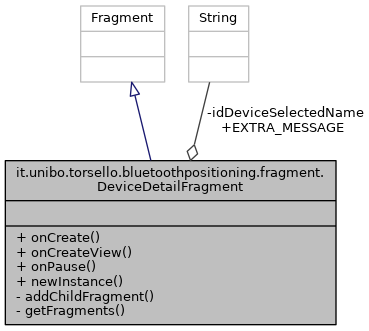
\includegraphics[width=0.7\linewidth]{img/uml/class/classit_1_1unibo_1_1torsello_1_1bluetoothpositioning_1_1fragment_1_1DeviceDetailFragment__coll__graph.png}
	\caption{Collaborazione - DeviceDetailFragment}
\end{figure}

\newpage
\section{CameraFragment}
\begin{figure}[ph]
	\centering
	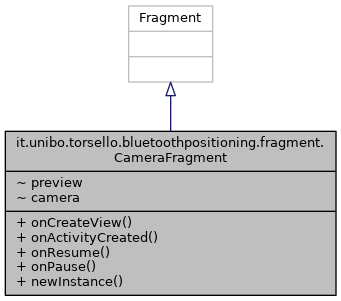
\includegraphics[width=0.5\linewidth]{img/uml/class/classit_1_1unibo_1_1torsello_1_1bluetoothpositioning_1_1fragment_1_1CameraFragment__inherit__graph.png}
	\caption{Classe - CameraFragment}
\end{figure}

Classe per implementare una SurfaceView come preview delle fotocamera presente nello smartphone e scattare delle foto (agli iBeacon). Per scattare le foto si è utilizzato un FloatingActionButton, mentre per fare l'autozoom basta cliccare sulla surface stessa.

\begin{figure}[ph]
	\centering
	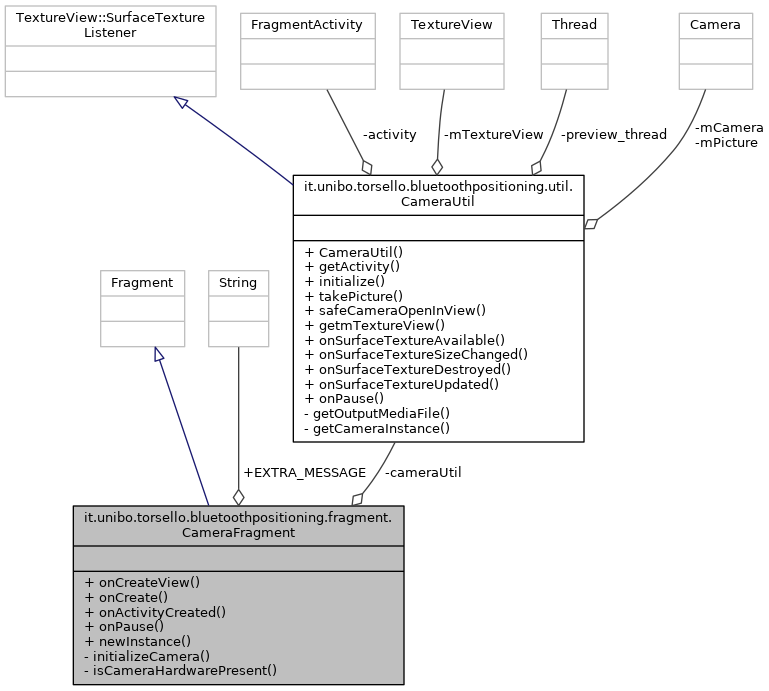
\includegraphics[width=1.5\linewidth, angle=90]{img/uml/class/classit_1_1unibo_1_1torsello_1_1bluetoothpositioning_1_1fragment_1_1CameraFragment__coll__graph.png}
	\caption{Collaborazione - CameraFragment}
\end{figure}

\newpage
\section{CameraPreviewUtil}
\begin{figure}[ph]
	\centering
	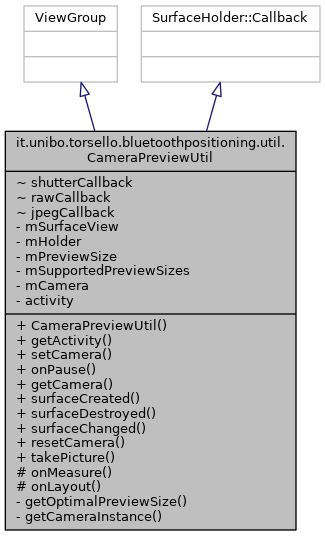
\includegraphics[width=0.5\linewidth]{img/uml/class/classit_1_1unibo_1_1torsello_1_1bluetoothpositioning_1_1util_1_1CameraPreviewUtil__inherit__graph.png}
	\caption{Classe - CameraPreviewUtil}
\end{figure}

Classe che controlla la SurfaceView di preview delle fotocamera e la telecamera stessa. Viene istanziata in \texttt{CameraFragment}.

\begin{figure}[ph]
	\centering
	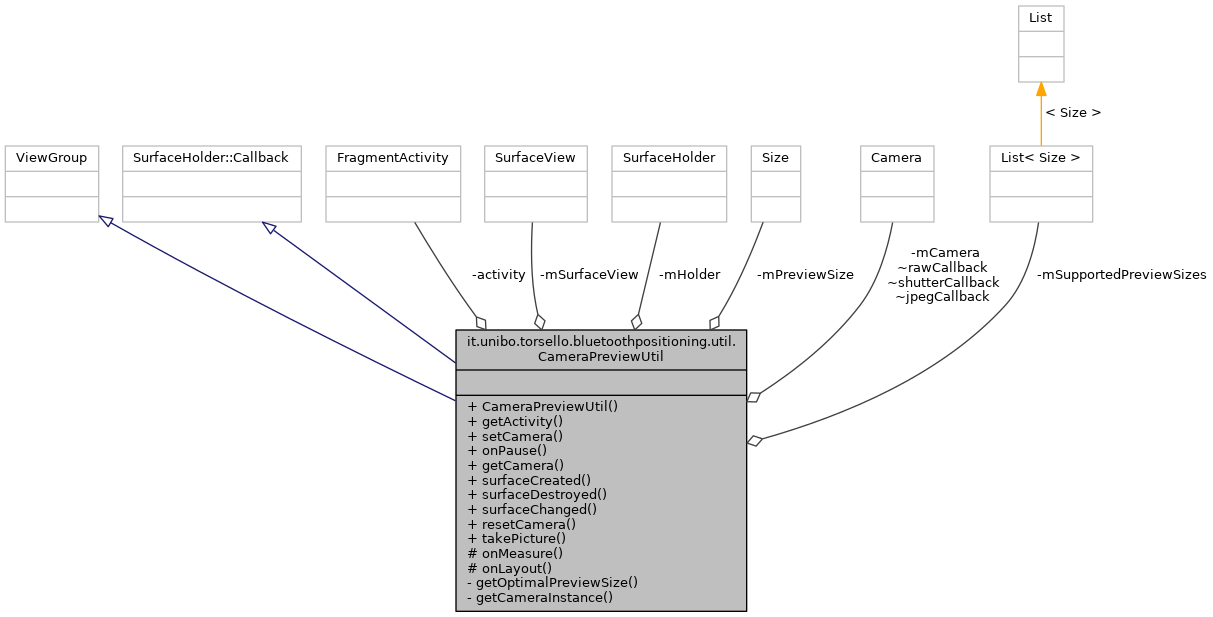
\includegraphics[width=1.5\linewidth,angle=90]{img/uml/class/classit_1_1unibo_1_1torsello_1_1bluetoothpositioning_1_1util_1_1CameraPreviewUtil__coll__graph.png}
	\caption{Collaborazione - CameraPreviewUtil}
\end{figure}

\newpage
\section{SaveImageTask}
\begin{figure}[ph]
	\centering
	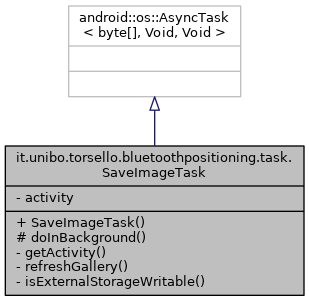
\includegraphics[width=0.5\linewidth]{img/uml/class/classit_1_1unibo_1_1torsello_1_1bluetoothpositioning_1_1task_1_1SaveImageTask__inherit__graph.png}
	\caption{Classe - SaveImageTask}
\end{figure}

Classe che serve a salvare le foto scattate dalla fotocamera. Implementa un AsyncTask per evitare che la GUI di Android si blocchi durante l'elaborazione dell'immagine.

\begin{figure}[ph]
	\centering
	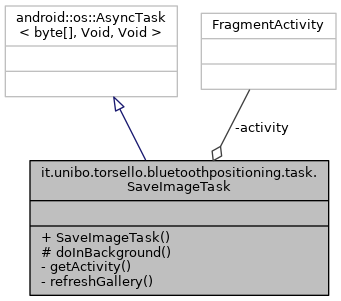
\includegraphics[width=0.5\linewidth]{img/uml/class/classit_1_1unibo_1_1torsello_1_1bluetoothpositioning_1_1task_1_1SaveImageTask__coll__graph.png}
	\caption{Collaborazione - SaveImageTask}
\end{figure}

\newpage
\section{DeviceDetailInner1Fragment}
\begin{figure}[ph]
	\centering
	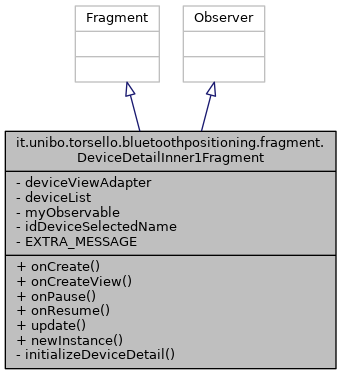
\includegraphics[width=0.6\linewidth]{img/uml/class/classit_1_1unibo_1_1torsello_1_1bluetoothpositioning_1_1fragment_1_1DeviceDetailInner1Fragment__inherit__graph.png}
	\caption{Classe - DeviceDetailInner1Fragment}
\end{figure}

Simile a \ref{ch:device_list}, aggiorna i dati di un solo beacon e visualizza la distanza dall'Arduino. Per la distanza stimata da Arduino si utilizza il fragment \texttt{UsbMeasurementFragment}, istanziato come fragment statico nel file XML.

\newpage
\section{DeviceDetailInner2Fragment}
\begin{figure}[ph]
	\centering
	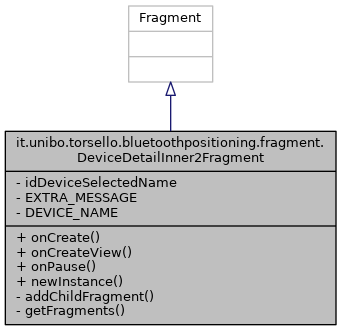
\includegraphics[width=0.5\linewidth]{img/uml/class/classit_1_1unibo_1_1torsello_1_1bluetoothpositioning_1_1fragment_1_1DeviceDetailInner2Fragment__inherit__graph.png}
	\caption{Classe - DeviceDetailInner2Fragment}
\end{figure}

Questa classe estende Fragment per inserire al proprio interno i dettagli dei beacon sotto forma di grafici in real time. L'obiettivo è permettere all'utente di controllare l'evoluzione del sistema e salvare i grafici sotto forma di immagini JPG.

\begin{figure}[ph]
	\centering
	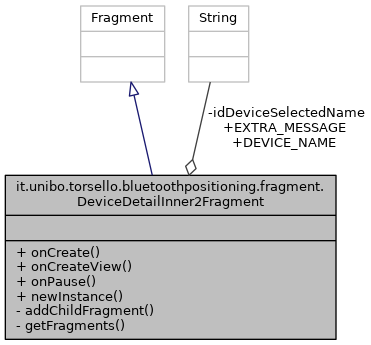
\includegraphics[width=0.55\linewidth]{img/uml/class/classit_1_1unibo_1_1torsello_1_1bluetoothpositioning_1_1fragment_1_1DeviceDetailInner2Fragment__coll__graph.png}
	\caption{Collaborazione - }
\end{figure}

\newpage
\section{DeviceChartFragment}
\begin{figure}[ph]
	\centering
	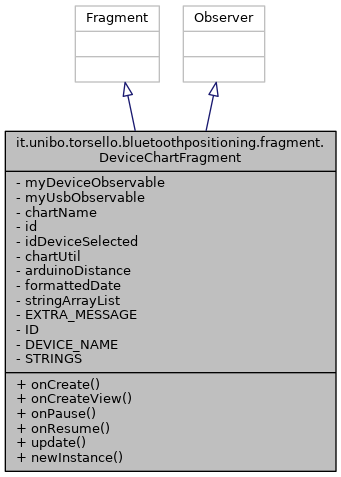
\includegraphics[width=0.5\linewidth]{img/uml/class/classit_1_1unibo_1_1torsello_1_1bluetoothpositioning_1_1fragment_1_1DeviceChartFragment__inherit__graph.png}
	\caption{Classe - DeviceChartFragment}
\end{figure}

Classe in cui si generano i grafici in realtime. I valori che vengono plottati sono le stime della distanza secondo Arduino e in base ai vari filtri su RSSI.

\newpage
\section{ChartUtil}

Classe per la creazione di grafici in real time. Viene sfuttata da \texttt{DeviceChartFragment} per istanziare un oggetto \texttt{LinearChart} a cui passare le varie distanze stimate via RSSI e USB.
\begin{figure}[ph]
	\centering
	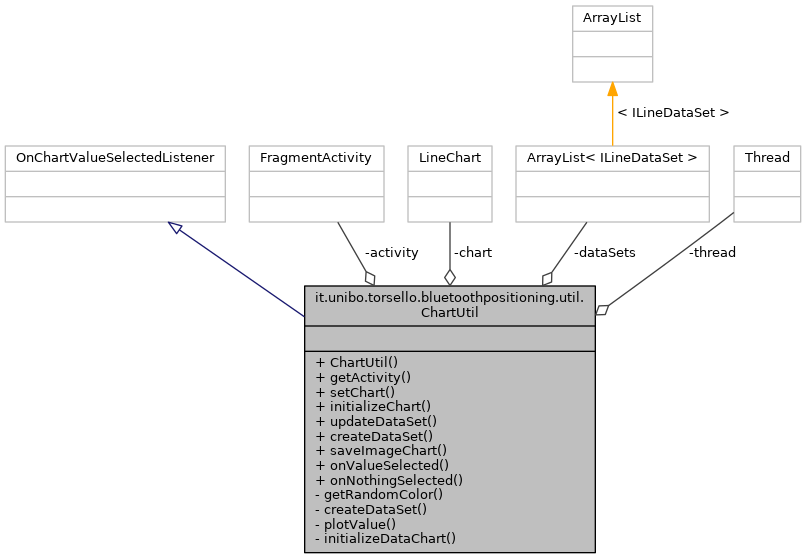
\includegraphics[width=1.2\linewidth]{img/uml/class/classit_1_1unibo_1_1torsello_1_1bluetoothpositioning_1_1util_1_1ChartUtil__coll__graph.png}
	\caption{}
\end{figure}

\newpage
\section{UsbMeasurementFragment}
\begin{figure}[ph]
	\centering
	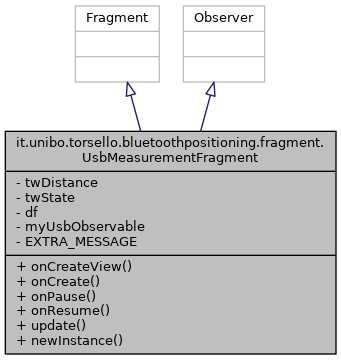
\includegraphics[width=0.5\linewidth]{img/uml/class/classit_1_1unibo_1_1torsello_1_1bluetoothpositioning_1_1fragment_1_1UsbMeasurementFragment__inherit__graph.png}
	\caption{Classe - UsbMeasurementFragment}
\end{figure}

Classe che visualizza su di un fragment i valori di distanza stimati dall'Arduino. Questa visualizzazione viene riutilizzata da sola se si seleziona "Measurement" dal menu a sinistra che nei dettagli. Nel caso dei dettagli il fragment è istanziato come statico dal file XML come segue:

\begin{lstlisting}[language=XML]
<android.support.v7.widget.CardView android:layout_width="match_parent"	android:layout_height="wrap_content" android:layout_margin="@dimen/card_margin">

	<fragment android:layout_width="match_parent" android:layout_height="wrap_content" android:name="it.unibo.torsello.bluetoothpositioning
	.fragment.usbObservers.UsbMeasurementFragment" android:id="@+id/usbArduino" tools:layout="@layout/fragment_usb_measurement" />
</android.support.v7.widget.CardView>
\end{lstlisting}

\begin{figure}[ph]
	\centering
	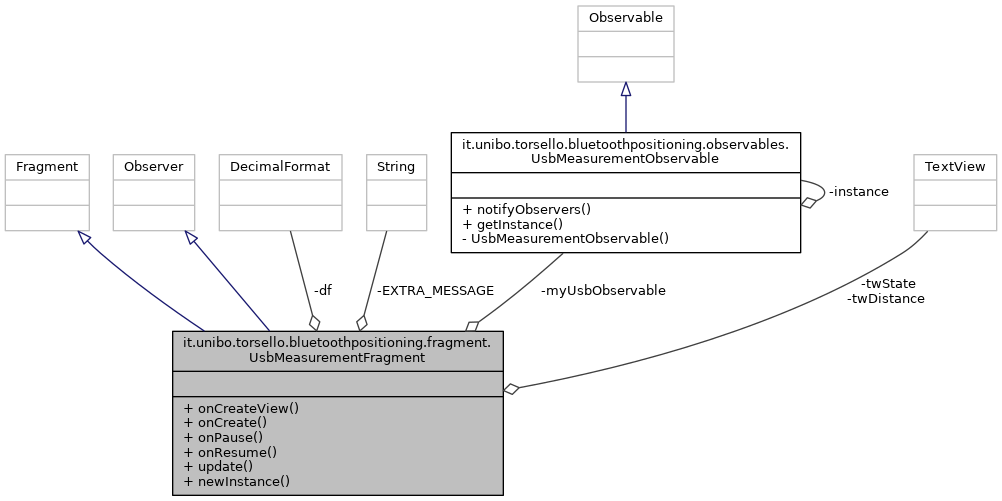
\includegraphics[width=1.6\linewidth,angle=90]{img/uml/class/classit_1_1unibo_1_1torsello_1_1bluetoothpositioning_1_1fragment_1_1UsbMeasurementFragment__coll__graph.png}
	\caption{Collaborazione - UsbMeasurementFragment}
\end{figure}

\newpage
\section{UsbUtil}

Classe che permette di comunicare con la porta USB dello smartphone e in questo caso di ricevere i dati della distanza stimata da Arduino. 

Per inizializzare la comunicazione su USB si utilizza il metodo \texttt{initializeUsb()}
\subsubsection{Metodo initializeUsb()}
\begin{lstlisting}[language=Java]
private void initializeUsb() {
	
	// Find all available drivers from attached devices.
	UsbManager usbManager = (UsbManager) getActivity().getSystemService(Context.USB_SERVICE);
	List<UsbSerialDriver> availableDrivers = UsbSerialProber.getDefaultProber()
		.findAllDrivers(usbManager);
		
	if (!availableDrivers.isEmpty()) {
		
		// Open a connection to the first available driver.
		UsbSerialDriver driver = availableDrivers.get(0);
		
		if (usbManager.hasPermission(driver.getDevice())) {
			if (usbManager.openDevice(driver.getDevice()) != null) {
				// Read some data! Most have just one port (port 0).
				port = driver.getPorts().get(0);
			}
		} else {
			Intent startIntent = new Intent(getActivity(), getClass());
			PendingIntent pendingIntent =
				PendingIntent.getService(getActivity(), 0, startIntent, 0);
			usbManager.requestPermission(driver.getDevice(), pendingIntent);
		}
		
		if (port != null) {
			
			UsbDeviceConnection connection = 
				usbManager.openDevice(port.getDriver()
					.getDevice());
			
			if (connection != null) {
				try {
					port.open(connection);
					port.setParameters(BOUND_RATE, UsbSerialPort.DATABITS_8,
					UsbSerialPort.STOPBITS_1, UsbSerialPort.PARITY_NONE);
				} catch (IOException e) {
					myUsbObservable.notifyObservers(getActivity()
						.getString(R.string.error_opening_device)
						+ " " + e.getMessage());
					myUsbObservable.notifyObservers(false);
					closePort();
					return;
				}
				
				stopIoManager();
				startIoManager();
			}
		}
	}
}
\end{lstlisting}

\begin{figure}[ph]
	\centering
	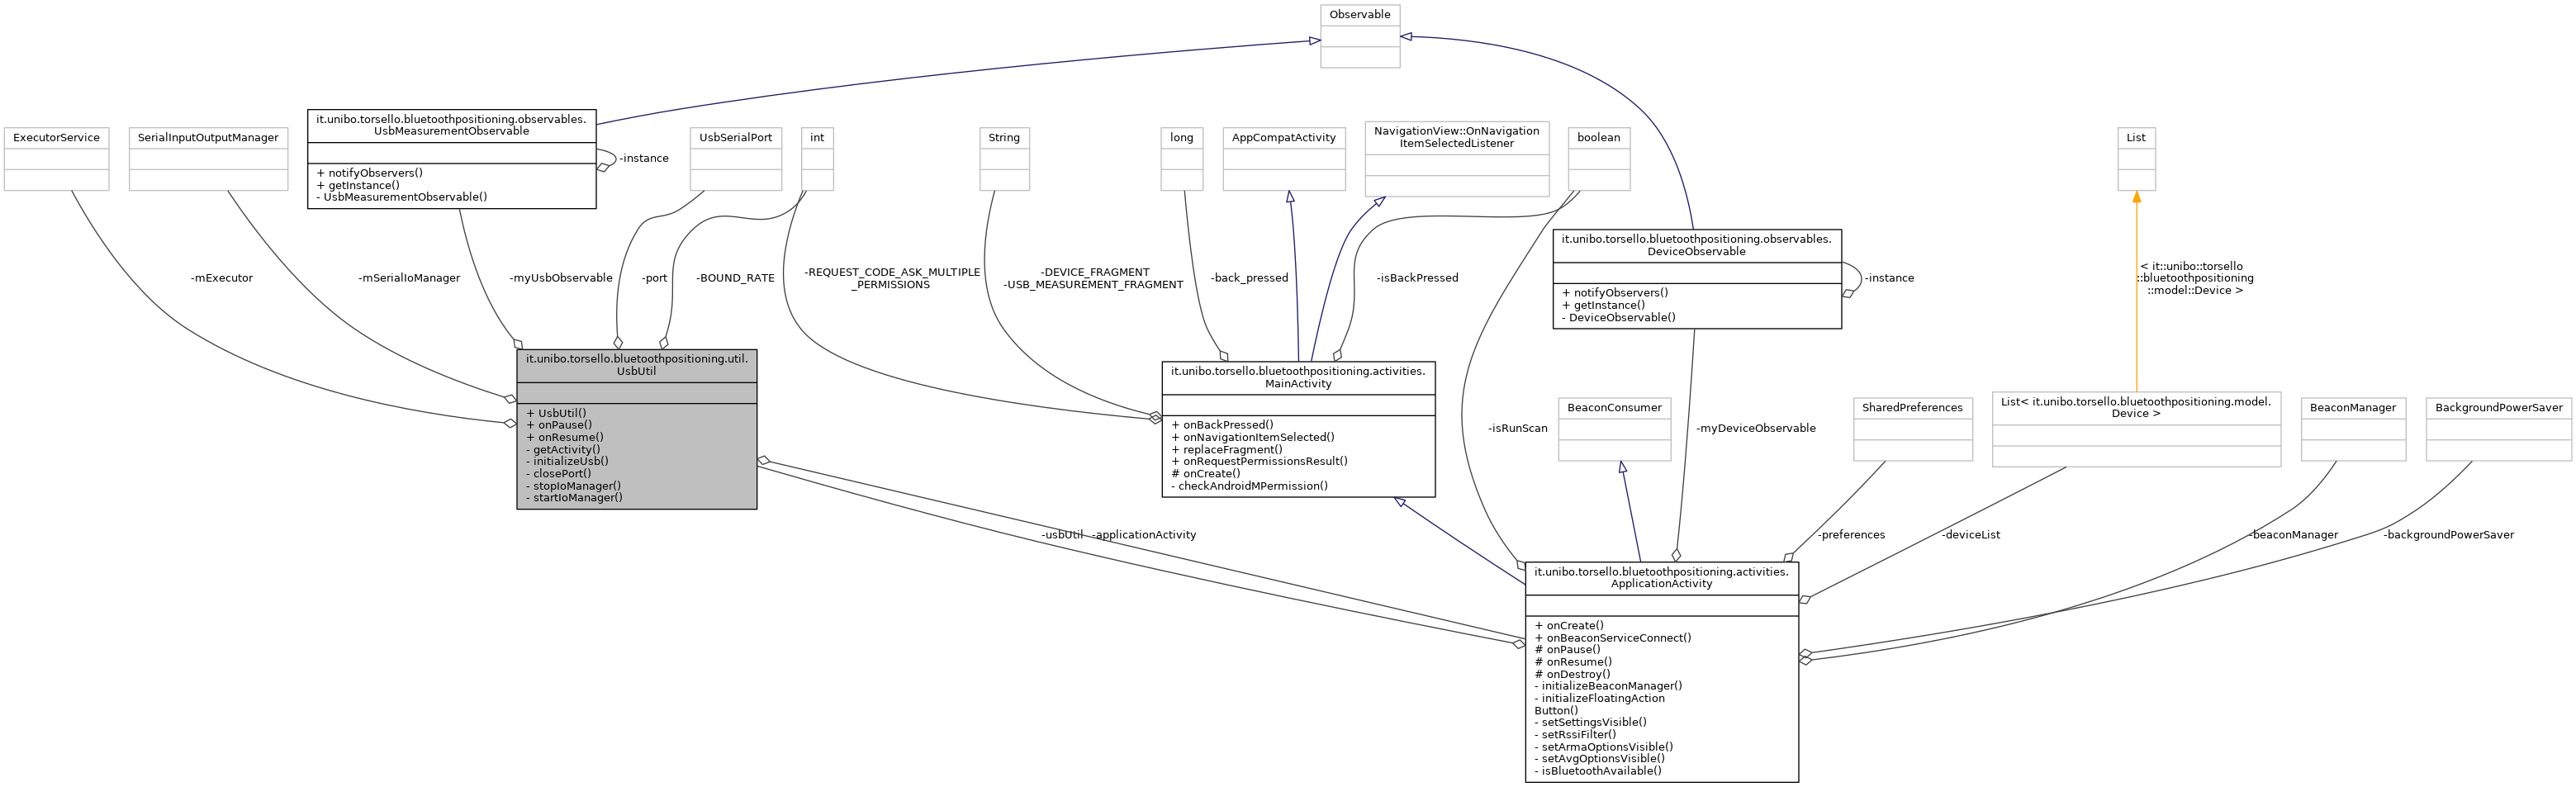
\includegraphics[width=1.85\linewidth,angle=90]{img/uml/class/classit_1_1unibo_1_1torsello_1_1bluetoothpositioning_1_1util_1_1UsbUtil__coll__graph.png}
	\caption{Collaborazione - UsbUtil}
\end{figure}

\newpage
\section{UsbMeasurementObservable}
\begin{figure}[ph]
	\centering
	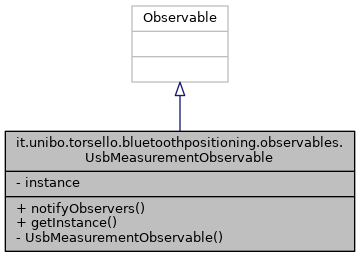
\includegraphics[width=0.6\linewidth]{img/uml/class/classit_1_1unibo_1_1torsello_1_1bluetoothpositioning_1_1observables_1_1UsbMeasurementObservable__inherit__graph.png}
	\caption{Classe - UsbMeasurementObservable}
\end{figure}

Classe Observable che emette le distanze stimate da Arduino a tutti gli Observer a lui registrati.

\begin{figure}[ph]
	\centering
	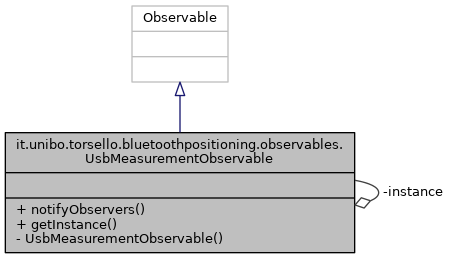
\includegraphics[width=0.8\linewidth]{img/uml/class/classit_1_1unibo_1_1torsello_1_1bluetoothpositioning_1_1observables_1_1UsbMeasurementObservable__coll__graph.png}
	\caption{Collaborazione - UsbMeasurementObservable}
\end{figure}

\newpage
\section{FABBehavior}
\begin{figure}[ph]
	\centering
	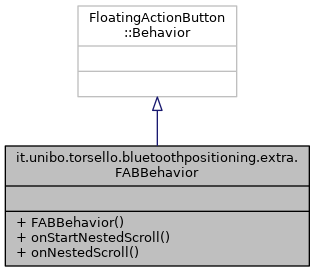
\includegraphics[width=0.6\linewidth]{img/uml/class/classit_1_1unibo_1_1torsello_1_1bluetoothpositioning_1_1extra_1_1FABBehavior__inherit__graph.png}
	\caption{Classe - FABBehavior}
\end{figure}

Classe che amplia il comportamento del FloatingActionButton in basso a destra, facendolo scomparire per un secondo quando una RecyclerView viene scrollata in alto o in basso.
Per funzionare si è dovuto modificare il file XML in cui il FAB è inserito con la regola \texttt{app:layout\_behavior=".extra.FABBehavior"}.